\section{逐次结果与复现补充}
图\ref{fig:matrix}显示全部48个范围内输入--重复单元在五臂的二元结果。
每四行对应一个构造条件，包含两个输入规模及两次重复；灰色不合格项没有被删除或最佳重试替换。
逐次JSON记录还保留失败字段、实际输入输出token和响应指纹。

\begin{figure*}[t]
\centering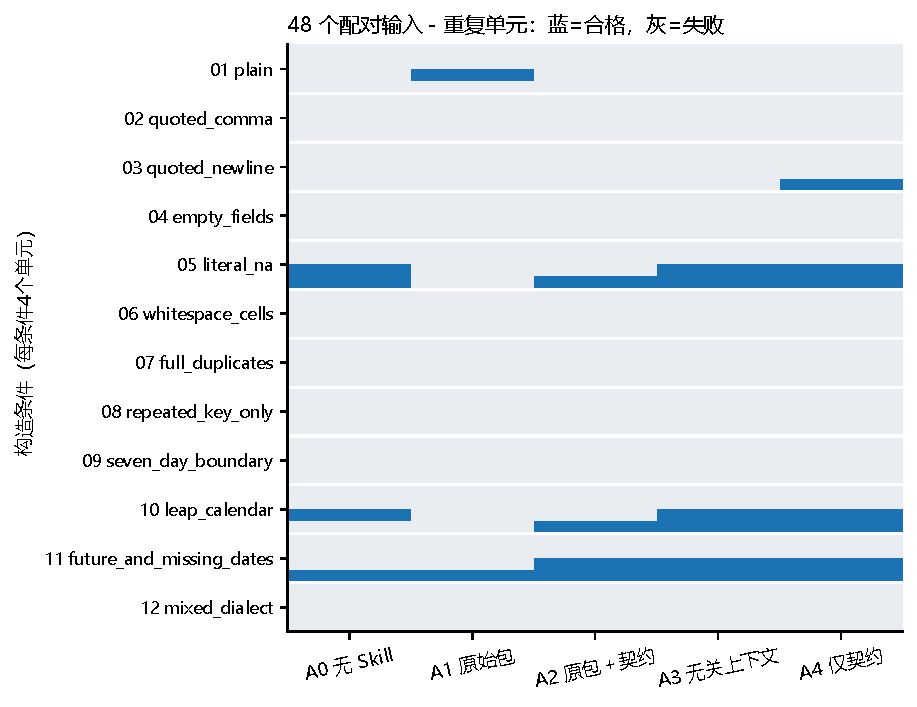
\includegraphics[width=.8\textwidth]{figures/artifact_matrix.pdf}
\caption{240份范围内实际产物的完整二元结果矩阵。数据为构造输入上的真实API输出；蓝色表示所有必需检查通过，灰色表示至少一项失败。条件排列在生成时固定，不按结果排序。}
\label{fig:matrix}
\end{figure*}

\subsection{输入与验收规则}
每个CSV包含 \texttt{id}、\texttt{amount}、\texttt{observed\_at}、\texttt{note} 四列。
构造输入的随机种子为20261111；闰年条件的基准日为2024-03-02，其余为2026-11-11。
原始记录的年龄变量保留于参考构造过程，序列化后经两个读取实现重新计算。
输入哈希由任务适配器提供供执行器复制，不把生成SHA-256作为能力测试。
每次请求是独立会话；执行器不会获得预期计数、验收代码或其他臂的答案。

对非完成状态，五个数据指标必须为空、操作列表为空，且状态须符合任务前提。
对完成状态，额外字段、缺字段、错误数值类型或任一错误指标均使完整任务失败。
这使正确格式、正确处置与正确测量分别可解释，同时防止全拒绝取得表面优胜。

\newpage
\subsection{代码与排版的验证}
新增构造任务及预算守卫通过专项检查，旧研究数据和源码指纹保留。
前期真实评价后曾修正跨平台类型标注，原始执行源码单独保存在代码快照中，
修正前后可执行语法树相同，未重复计入模型请求。
本文使用Elsevier CAS双栏类2.4和中文排版支持，由用户指定的TeX Live 2026中的XeLaTeX编译。
该模板提供版式，不代表目标期刊适配、录用状态或研究结论的权威性。

\subsection{不应从本文推出的结论}
不能将154个机械缺陷全检出写成所有技能100\%准确；
不能将来源窗口全部绑定写成语义判断全部正确；
不能将60次明确边界处置正确写成操作系统或真实二进制格式安全；
不能将观察成功数最高的方法写成跨技能、跨模型最优；
也不能将检索覆盖写成实际编排成功率。
这些限制是测量对象的一部分，而不是在结果产生后删去失败的理由。

\subsection{新网络的逐源与逐任务核对}
\begin{figure*}[p]
\begin{minipage}[t]{.48\textwidth}\vspace{0pt}
\localtablecaption{主结果分数据集核对。每格为同64个输入在三档预算下的成功总数/192。两个数据集的模式完全相同，反映构造语义主导的限制。}\label{tab:network-datasets}
\centering\small
\begin{tabularx}{\columnwidth}{Xrr}
\toprule
策略 & WDBC & Banknote \\
\midrule
词法前五＋路径 & 12/192 & 12/192 \\
MMR 前五＋路径 & 60/192 & 60/192 \\
DPP 前五＋路径 & 60/192 & 60/192 \\
原生元数据最短路径 & 24/192 & 24/192 \\
人工固定流程 & 128/192 & 128/192 \\
全局证据过滤＋最短路径 & 64/192 & 64/192 \\
全局证据风险路径 & 128/192 & 128/192 \\
ECP 完整方法 & 136/192 & 136/192 \\
条件证据前五＋路径 & 90/192 & 90/192 \\
ECP 去版本绑定 & 136/192 & 136/192 \\
\bottomrule
\end{tabularx}

\vspace{8mm}\raggedright\small
主留出只包含128个不同输入，每个数据集64个。表中192为64个输入乘三档预算；两个数据集同样的成功总数不代表192个独立任务，也不能用重复预算缩窄区间。

\medskip
原始记录位置：\texttt{research/skill\_network/results/} 下的 \texttt{prepared-v3}、\texttt{calibration-v2}、\texttt{execution-v2}、\texttt{analysis-v1} 和 \texttt{joint-posthoc-v1}。
公开元数据、执行前选择、worker请求、原始输出和逐项判定分别保存，便于审查是否发生答案泄漏或失败删除。

\medskip
完整复现同时检查原始源文件指纹、开发/留出隔离、逐次选择、全部产物、三档聚合、条件重采样及事后反例。CI复现报告记录了无凭据、无网络及只读边界；它增加实现可移植性证据，不增加科学样本或领域认可。
\end{minipage}\hfill
\begin{minipage}[t]{.48\textwidth}\vspace{0pt}
\centering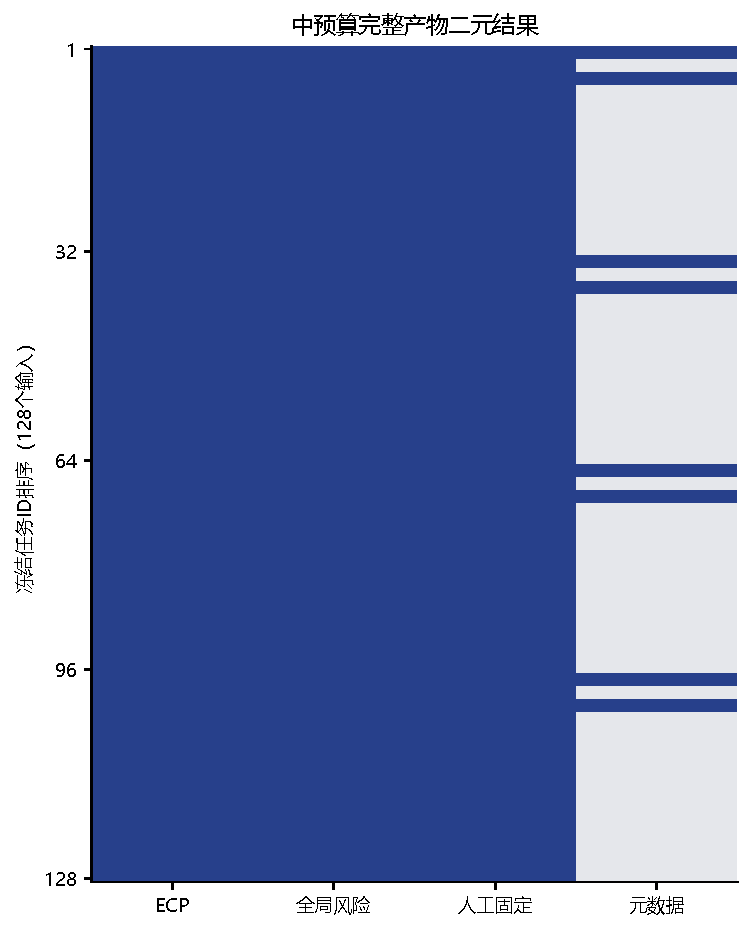
\includegraphics[width=.96\linewidth]{figures/network_binary_matrix.pdf}
\localfigurecaption{中预算128个主输入的二元完整成功矩阵。按冻结ID排序，蓝色为全部检查通过，灰色为失败或弃权；这里只显示四个预定代表策略，全部十策略记录随稿。}
\label{fig:network-matrix}
\end{minipage}
\end{figure*}

新网络的协议、代码快照和选择记录先于worker执行写出；原始冻结目录中的准备/校准路径名只标识历史运行，不作为外部预注册证明。
离线复现逐条重算7,856个主运行选择、240个事后选择和全部独立验收，再用同一随机种子重算区间。
可选重执行合并928次开发探测、1,204条主路径及132条事后路径共2,264个worker请求，不增加独立样本。
